\begin{section}{Business Logic Layer}

\subsection{Design}

Der BusinessLogicLayer spiegelt die Kernkomponente der Drei-Schichten-Architektur und bindet die Datenzugriffsschicht mit dem Frontend UI. Hierfuer wurden folgende Basis-Interfaces verwendet.


IValidationAccessBll und IAuthAccessBll. Diese werden in ein Rollenkonzept fuer die Zugriffsberechtigungen wiederverwendet. Hierfuer wurden eine administrative und eine oeffentliche Rolle definiert, welche von IAdminAccessBll und IViewAccessBll abgeleitet werden. Darauf aufbauend wurde eine abstrakte Basisklasse realisiert, welche kommunale Funktionalitaeten implementiert. Von dieser Basisklasse werden nun die konkreten Instanzen wie, AdminAccessBll realisiert. Diese bietet die Funktionalitaet User-, Artist-Daten oder auch andere Domaenenobjekte nicht nur anzuzeigen, sondern auch zu modifizieren. Fuer den oeffentlichen Zugriff wurde eine Ableitung von der abstrakten Klasse AViewAccessBll implementiert, welche die oeffentlich verfuegbaren Daten bereitstellt.

Wie in der Spezifikation gefordert, wurde eine Login Moeglichkeit geschaffen, welche Serverseitig verwaltet wird. Die Applikation wurde dahingehend erweitert, dass mehrere Login-Instanzen unterstuetzt werden\; das heisst hierfuer wird ein serverseitiges Sessionhandling verwendet. Loggt sich beispielsweise ein User mit der Frontendapplikation ein, wird fuer Ihn eine Session am Server angelegt und sofern eine zweite Instanz von einem weiteren Client mit selben Authenifizierungsdaten angefragt wird, wird die erste Session gecancelt.




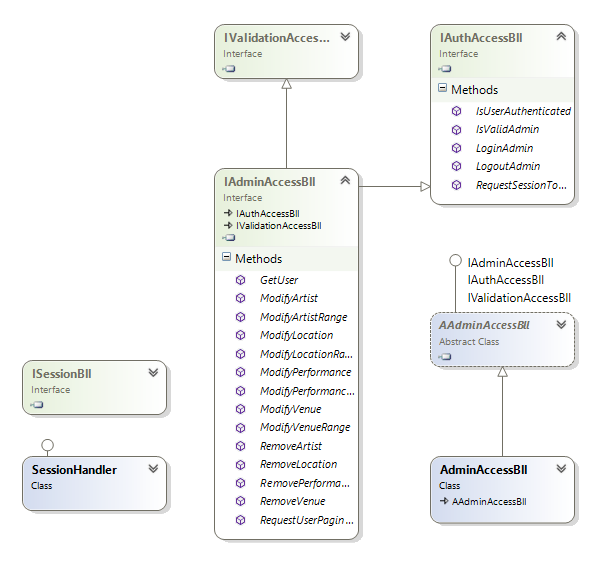
\includegraphics[angle=0, scale=0.45]{./img/blladminaccess.PNG}
\FloatBarrier
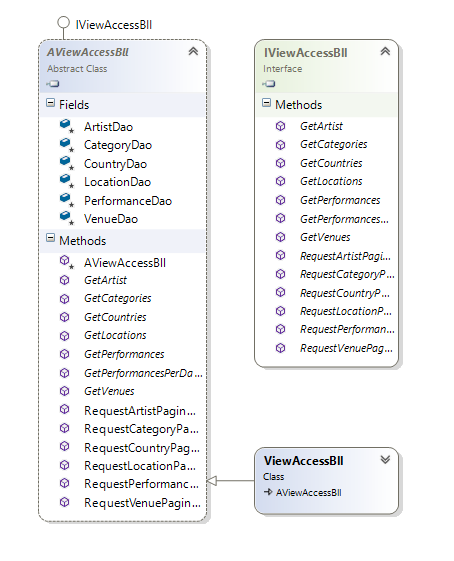
\includegraphics[angle=0, scale=0.45]{./img/bllviewaccess.PNG}
\FloatBarrier

Die Domaenenklassen wurden dahingehend erweitert, ein Sessionhandling zu unterstuetzen. Hierfuer wird die Klasse SessionToken als Transportobjekt verwendet. Hierfuer muss der Client an den Server einen Request mit den Authentifizierungsdaten senden und erhaelt bei einem gueltigen Request ein Sessionobjekt.
In Voraussicht auf die dritte Ausbaustufe und zu uebungszwecken wurde bereits hierfuer ein Webservice implementiert. Um Daten ueber das Webservice austauschen zu koennen, wurde das PagingData Objekt angelegt, damit die maximale Payload limitiert wird. Des Weiteren besitzen Webservices auch eine maximale Message Groesse.

Die im folgenden Diagramm ersichtlich, leiten alle Domaenenklassen von DomainObject ab. Der Grund hierfuer wird im nachfolgenden Kapitel naeher erlaeutert. 

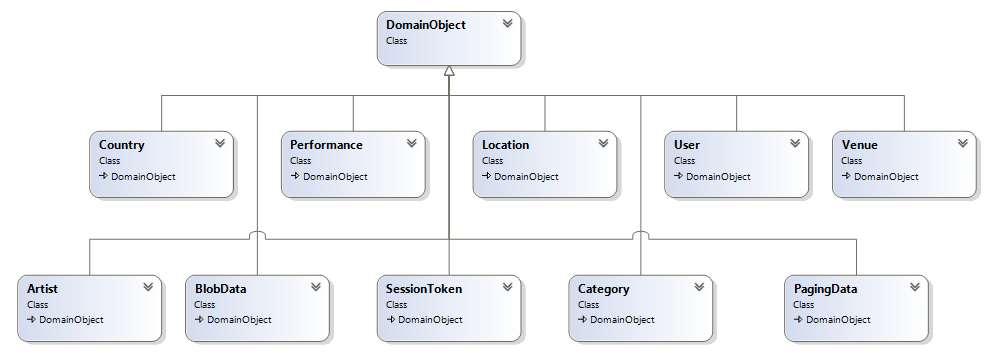
\includegraphics[angle=0, scale=0.45]{./img/domainclasses.PNG}
\FloatBarrier

\subsection{WebService}

Fuer die Webservice Realisierung wurde WCF verwendet, da sich Client und Server in derselben Technologiesprache CSharp implementiert sind. Der Webservice verwendet das SOAP basierte Transportprotokoll fuer Kommunikation. Die Clientklassen werden vom WSDL (serverseitigem Service) generiert. 
Um eine Abstraktionsschicht zwischen generierten Klassen und den im WPF Client verwendeten Funktionalen Klassen herzustellen, wurde ein Proxy assembly erstellt. Dieses bietet auch eine Erweiterung (Extension Methods) um Domaenenklassen zu Webserviceklassen (und vice versa) mappen zu koennen, da der Client nur mit den Domaenobjekten operieren soll, um Technologie unabhaengig zu fungieren. 
Im folgenden Beispiel wird eine Extensionmethod demonstrativ dargestellt. Diese nuetzen den Mechanismus der Reflexion, um von einer Klasse zu einer anderen Klasse mit gleichen Properties (Primitivtyp und Name sind equivalent) Daten zu mappen.

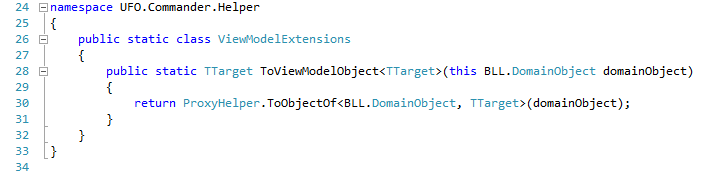
\includegraphics[angle=0, scale=0.45]{./img/domainclassesextension.PNG}
\FloatBarrier

Um zwischen dem Webservice und eventuell anderen Implementierungen wechseln zu koennen, wird das Factorypattern angewendet (BllFactory), welche die Instanziierung der darunterliegenden Schicht vornimmt.

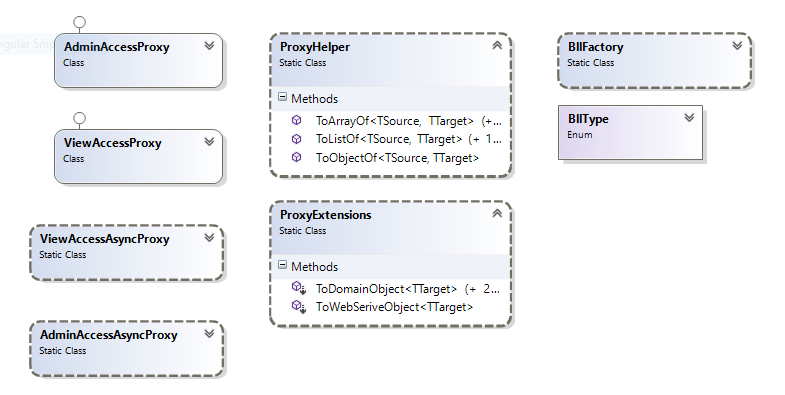
\includegraphics[angle=0, scale=0.45]{./img/proxy.PNG}
\FloatBarrier

Am Client wird an zentraler Stelle via Singleton auf die BllFactory zugegriffen.

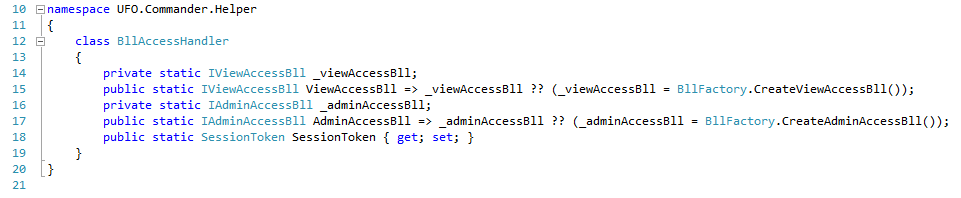
\includegraphics[angle=0, scale=0.45]{./img/proxyaccess.PNG}
\FloatBarrier

\end{section}


\begin{section}{WPF}
Fuer die Realisierung des MVVM Patterns, wurden zusaetzliche Softwarekomponenten (Frameworks) wie MahApps Metro, MVVM Light und Caliburn.Micro verwendet. Dabei fungiert MahApps Metro als UI-Framework fuer ein ansehnliches Look \& Feel des User-Interfaces. Caliburn.Micro hingegen erweitert die XAML Funktionalitaet und bietet beispielsweise ein komfortables Moeglichkeit fuer das Binding mit der TreeView Komponente, um das selektierte Element zu erhalten. MVVM Light wird verwendet um ViewModels via DataTemplates auf UI Komponenten projizieren zu koennen und per ServiceLocator ansprechen zu koennen. Das heisst konkret, dass Messages gesendet werden koennen, welche das als naechstes anzuzeigende ViewModel beinhaltet. Aus dieser kann die dazugehoerige View gemappt werden. 

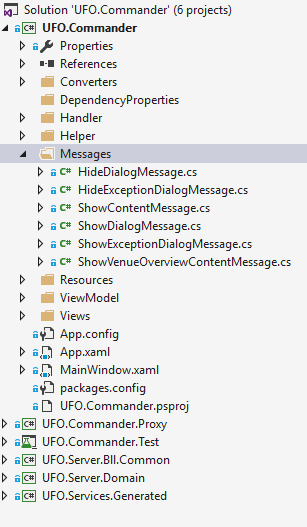
\includegraphics[angle=0, scale=0.45]{./img/messagesproject.PNG}
\FloatBarrier

Alle ViewModels werden vom Service Locator an zentraler Stelle verwaltet.

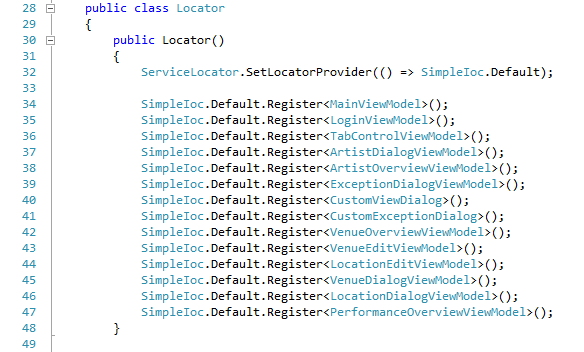
\includegraphics[angle=0, scale=0.45]{./img/servicelocator.PNG}
\FloatBarrier

Nun kann per Service Locator beispielsweise im XAML das benoetigte ViewModel fuer das DataContext-Binding verwendet werden.

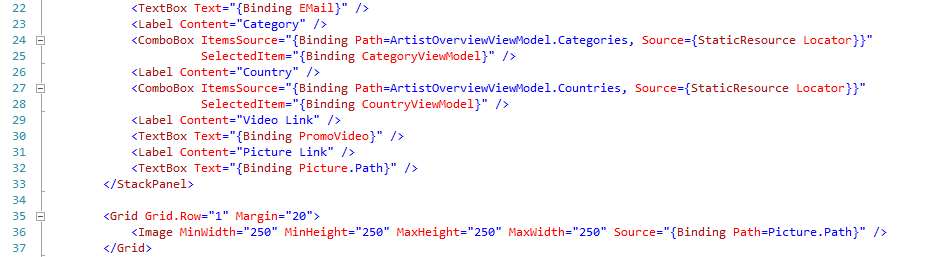
\includegraphics[angle=0, scale=0.45]{./img/servicelocatorusage.PNG}
\FloatBarrier

\subsection{ViewModels}

Wie in der folgenden Illustrierung erben alle ViewModel-Klassen von ViewModelBase, welche von MVVM Light bereitgestellt wird.

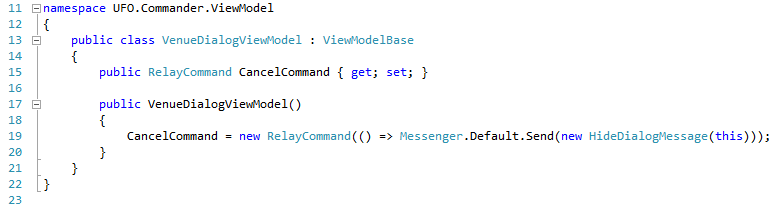
\includegraphics[angle=0, scale=0.45]{./img/messagescode.PNG}
\FloatBarrier

Fuer jede benoetige Doaenenklasse wurde ein dazugehoeriges ViewModel erstellt. Hierbei wurde von den Domaenenklassen abgeleitet, um via Attributen das NotifyPropertyChanged Event auf die Properties abbilden zu koennen.

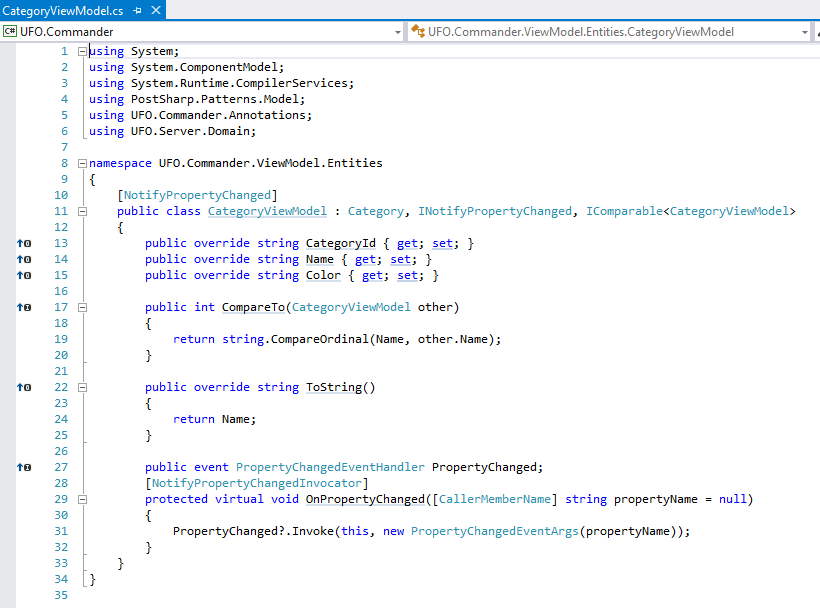
\includegraphics[angle=0, scale=0.45]{./img/categoryvmcode.PNG}
\FloatBarrier

\subsection{Exception Handling}
Das Exceptionhandling wird wie in der ersten Ausbaustufe durch Aspekt orientierte Attribute gesteuert und auf eine User-freundliche View via Messaging projeziert. 

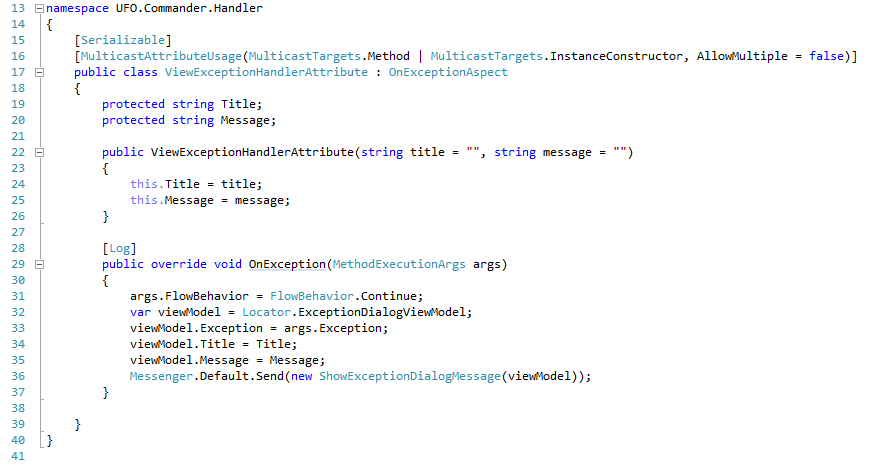
\includegraphics[angle=0, scale=0.45]{./img/exception.PNG}
\FloatBarrier

\end{section}

\begin{section}{User Interface}
Das User Interface verfuegt ueber drei Mainpages (Artists, Venues und Performances). Bevor mit diesen Pages interagiert werden kann, muss sich der User ueber den Login-Dialog authentifizieren. Alle Neu hinzuzufuegenden Eintraege werden auch per Dialog gesteuert. Existierende Eintraege koennen direkt, wie unten zu sehen ist, editiert werden.


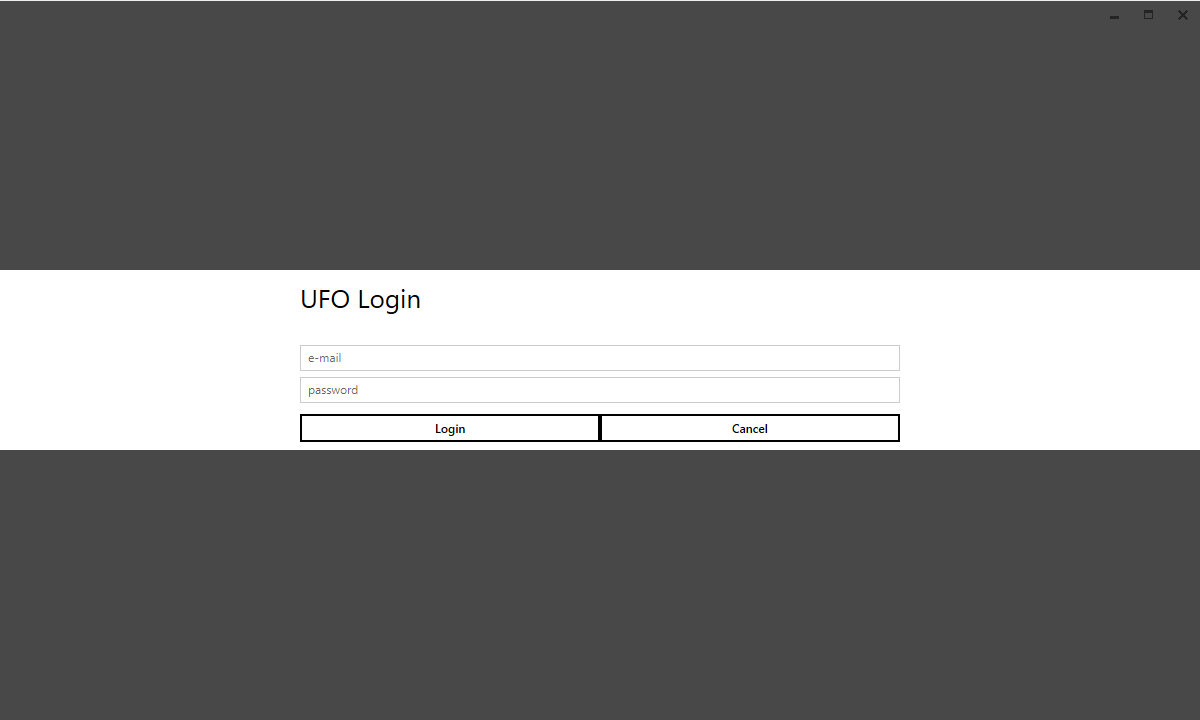
\includegraphics[angle=0, scale=0.45]{./img/viewlogin.PNG}
\FloatBarrier

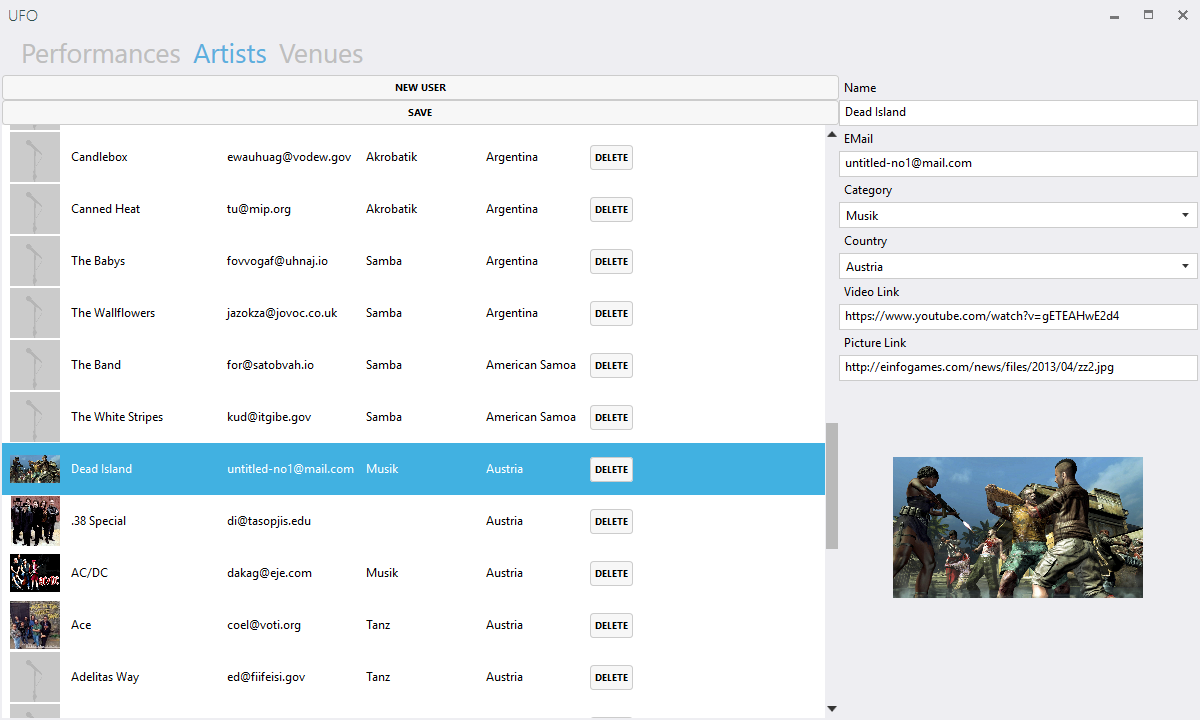
\includegraphics[angle=0, scale=0.45]{./img/viewartist.PNG}
\FloatBarrier

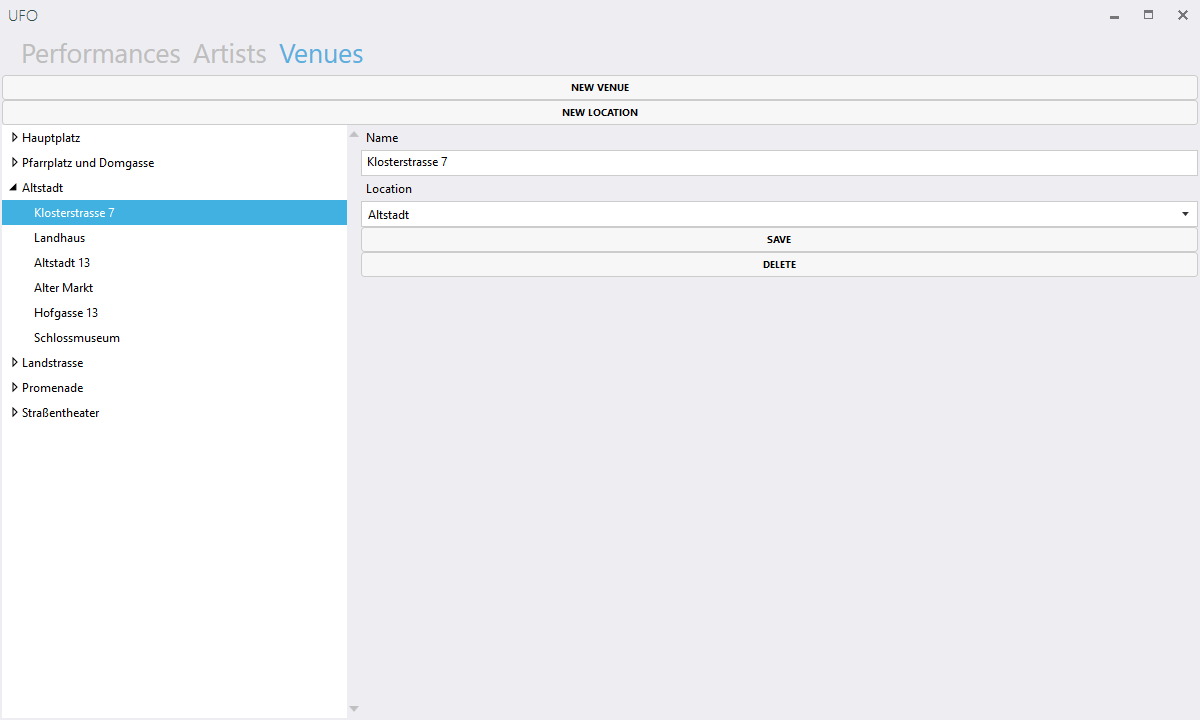
\includegraphics[angle=0, scale=0.45]{./img/viewvenue.PNG}
\FloatBarrier

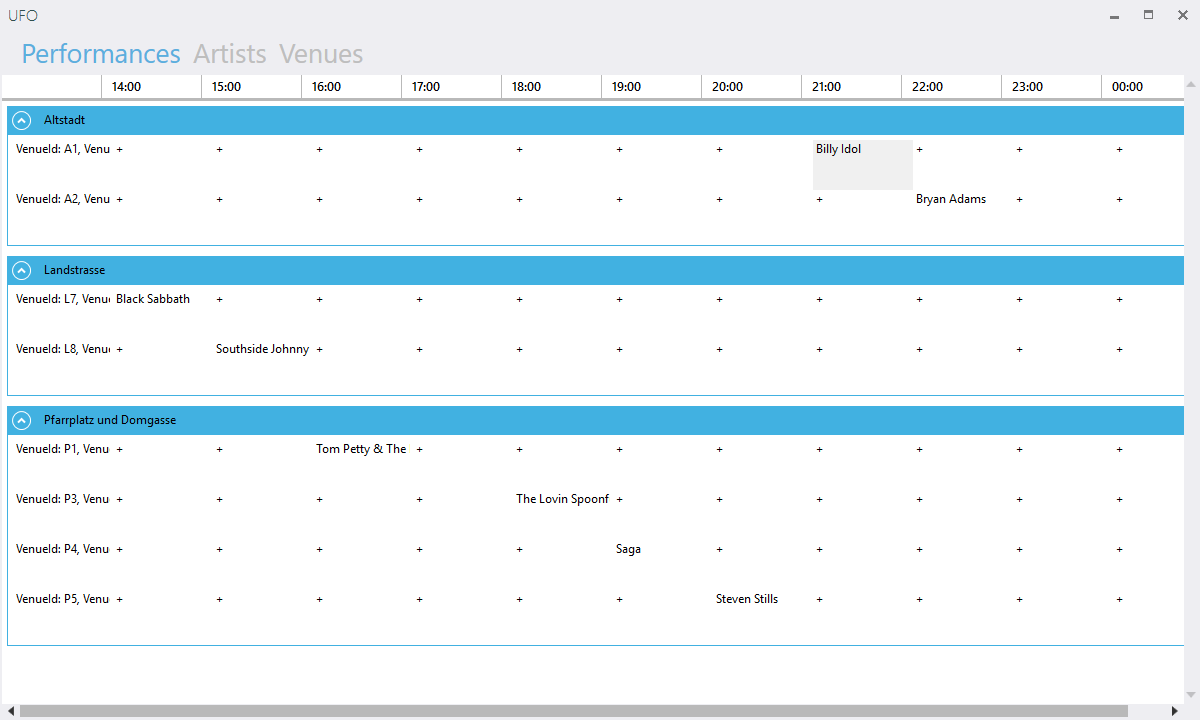
\includegraphics[angle=0, scale=0.45]{./img/viewperformance.PNG}
\FloatBarrier


\end{section}